\documentclass[12pt,a4paper,twoside,%
BCOR12mm,DIV12,%
headsepline,%
cleardoubleempty,chapterprefix,parskip,%
liststotoc,idxtotoc,bibtotoc]{scrbook}

\usepackage[english, ngerman]{babel}
\usepackage[utf8]{inputenc}
\usepackage[T1]{fontenc}
\usepackage{mathptmx}
\usepackage[scaled=0.92]{helvet}
\usepackage{courier}
\usepackage{amsmath}
\makeatletter
\def\displaymath{\typeout{*** Do not use DISPLAYMATH. Use \[...\] instead ***}}
\def\eqnarray{\typeout{*** Do not use EQNARRAY(*). Use align(*)-environment instead ***}}
\makeatother
\usepackage{amsfonts}
\usepackage{amstext}
\usepackage{subfigure}
\usepackage{color}
\usepackage{wrapfig}	% let text float around pictures
\usepackage{graphicx}
\usepackage{ifpdf}
\usepackage{makeidx}
\usepackage{nomencl}
\usepackage{setspace}

\usepackage{listings}

% first include hyperref, then cite
\usepackage[plainpages=false,pdfpagelabels]{hyperref}
\usepackage{cite}

\usepackage{lscape}
\usepackage{tabularx}

\ifpdf
    \definecolor{brown}{cmyk}{0, 0.81, 1, 0.60}
    \hypersetup{%
      pdftitle={Verteiltes Veranstaltungsmanagement mit einer mobilen Webanwendung}, %%%% HIER AENDERN!!!
      pdfsubject={Bachelorarbeit},
      pdfauthor={Christian Meter},           %%%% HIER AENDERN!!!
      pdfkeywords={KEYWORDS},      %%%% HIER AENDERN!!!
      colorlinks=false, urlcolor=blue, citecolor=brown,
      bookmarksnumbered=true,
    }
\else   
\fi

\listfiles

\begin{document}
\onehalfspacing

\frontmatter

\pdfbookmark[0]{Titelseite}{tit}
% Titelseite

\begin{titlepage}
  \centering
  \includegraphics[width=5cm]{fig/unilogo}\\

  \vfill
  \huge
  Installations- und Bedienungsanleitung\\für die Meißner Webanwendung\\*[40pt]
  \normalsize

  \vfill
  \large
  \normalsize
  von\\
  \Large
  Christian Meter
    
\end{titlepage}


%%% Local Variables: 
%%% mode: latex
%%% TeX-master: "master"
%%% End: 


\cleardoublepage

\pdfbookmark[0]{Abstract}{abstract}
\begin{center} 
\huge Abstract
\end{center}

Hier beschreibe ich nun auf einer Seite, welches Problem ich betrachtet, wie ich es gelöst habe
und was die Hauptergebnisse meiner Arbeit sind.

Entwicklung einer Webanwendung, die das Verwalten von Veranstaltungen mit vielen Benutzern und Helfern ermöglicht. Touchoptimierte Seiten für mobile Endgeräte ermöglichen eine einfache Handhabung und bieten den gleichen Funktionsumfang wie die Desktopanwendung.\par

Die Meißner App ist für die Nutzung im Außenbereich auf einer großen Fläche gedacht, weshalb über eine Echtzeitaktualisierung mit WebSockets den Austausch der Geolocations einzelner Endgeräte ermöglicht wird. Dadurch können die Standorte der Helfer erfragt werden und diese dann effektiver durch Wegoptimierung eingesetzt werden.\par

Eigene Module für PUSH-Benachrichtigungen und der Möglichkeit einzelne Veranstaltungen zu abonnieren wurden implementiert. 

Kurze Zusammenfassung (ca. 200 Wörter)\\
* Klar und prägnant: Worum gehts? Was wurde herausgefunden? Warum ist das wichtig?\\
* Aushängeschild des Artikels; Reviewer bilden sich eine Meinung, Leser entscheiden, ob der Artikel für sie relevant ist\\
* Abstract dient als Gedächtnisstutze (Worum gings nochmal in dem Paper?)



\cleardoublepage

\pdfbookmark[0]{Danksagungen}{ack}
\begin{center} 
	\huge Danksagungen
\end{center}
Mit vielen Leuten konnte ich wichtige Gespräche führen, die mir thematisch und inhaltlich sehr weitergeholen haben. Daher danke ich allen, die mich bei dieser Arbeit unterstützt haben.\par

Ein besonderer Dank gilt meinem Betreuer der Bachelorarbeit Philipp Hagemeister, welcher immer ein offenes Ohr hatte und mir stets geholfen hat. Vielen Dank dafür.

\cleardoublepage

\pdfbookmark[0]{\contentsname}{content}
\tableofcontents

\listoffigures

%\listoftables

%\lstlistoflistings

\mainmatter

\cleardoublepage

%%%%%%%%%%%%%%%%%%%%%%%%%%%%%%%%%%%%%%%%%%%%%%
%%    Beginning of the main document        %%
%%                                          %%
%%    Include your tex-files with \input{}  %%
%%%%%%%%%%%%%%%%%%%%%%%%%%%%%%%%%%%%%%%%%%%%%%

\chapter{Voraussetzungen}
Getestet wurde diese Installation auf einer frischen Installation von Debian. Dieses Installationsskript ist auch ausschließlich unter Distributionen lauffähig, die \emph{apt-get} verwenden.

\chapter{Installation eines Webservers}
\paragraph{LAMP}
LAMP steht für \emph{Linux, Apache, MySQL, PHP} und stellt die Basis eines einfachen Webservers dar.\par

Die Installation wird mit 

\begin{lstlisting}
	sudo sh install.sh
\end{lstlisting}

begonnen.

\begin{figure}[!ht]
	\centering
	\includegraphics[width=15cm]{fig/configuring_mysql}
	\caption{Eingabe des root Passworts für die MySQL Datenbank}
\end{figure}

\begin{figure}[!ht]
	\centering
	\includegraphics[width=15cm]{fig/configure_phpmyadmin}
	\caption{Eingabe des root Passworts für phpmyadmin}
\end{figure}



\chapter{Theoretischer Hintergrund}
TODO: Einleitung für das Kapitel schreiben

\section{Definition: Webanwendung}
Eine Webanwendung (auch \emph{Web-App} genannt) ist eine Anwendung, die vollständig in einem Browser ausführbar ist. Da sie (fast) vollständig auf einem Webserver ausgeführt wird, ist das zugrunde liegende Übertragungsprotokoll \emph{HTTP}.\par

Web-Apps bieten den Vorteil, dass sie in jedem modernen Browser ausgeführt werden können, ohne, dass spezielle Programmiersprachen erlernt und angewendet werden müssen. Interessant sind diese Anwendungen, da sie auch auf Smartphones und Tablets ausgeführt werden können ohne sie vollständig auf die jeweilige Plattform portieren zu müssen.

\section{Verwendete Programme, Anwendungen und Programmiersprachen}
\subsection{HTML5}
\subsection{cakePHP}
\subsection{XAMPP}
\subsection{jQuery und jQuery Mobile}

\chapter{Implementierung}
\paragraph{Identifizierung des Problems}
Bei dem Gedanken eine App zu entwickeln, steht man oft vor der Entscheidung für welche Plattform man denn entwickeln möchte: Linux, Windows, OS X, iOS, Android, Windows Phone, Blackberry OS etc. Doch das würde voraussetzen, dass alle Benutzer dieser App das gleiche Betriebssystem benutzen. Für eine Veranstaltung, wie das Meißnerlager, eine sehr schlechte Annahme. Die ehrenamtlichen Helfer müssen mit ihren eigenen / privaten Smartphones und Tablets arbeiten. Es ist davon auszugehen, dass es sich dabei um unterschiedliche Geräte mit verschiedenen Betriebssystemen handelt.\par

Wieso also nicht für alle Plattformen gleichermaßen entwickeln? Dank dem Google Projekt \glqq HTML5 Rocks\grqq{}\cite{html5rocksmain} und vielen interessierten Entwicklern ist \emph{HTML5} in aller Munde. Somit gibt es tatsächlich die Möglichkeit, jedes Betriebssystem mit einer einzigen Webanwendung abzudecken.

\paragraph{Definition Webanwendung} 
Eine Webanwendung, auch \emph{Web-App} genannt, ist eine Anwendung, die vollständig in einem Browser ausführbar ist. Da sie (fast) vollständig auf einem Webserver ausgeführt wird, ist das zugrunde liegende Übertragungsprotokoll \emph{HTTP}.\par

Das Interessante an dieser Art der Anwendungen ist, dass sie auch auf Smartphones und Tablets ausgeführt werden können, ohne sie vollständig auf die jeweilige Plattform portieren zu müssen. Das heißt, man entwickelt einmal eine Webanwendung und kann sie dann auf allen gängigen Endgeräten ausführen.\\
Damit wäre ein wichtiges Kriterium für die Nutzung beim Meißner erfüllt: die betriebssystemunabhängige Nutzung.

\paragraph{Auszeichnungssprache HTML5}
\emph{HTML5} ist der angehende Nachfolger des aktuell verwendeten HTML 4.0.1. Es ist immer noch im experimentellen Entwicklungsstand, wird aber durch große Unternehmen wie Google gefördert und erreichte damit auch eine große Beliebtheit. Alle Browser verstehen die gängigsten HTML5 Befehle, allerdings werden nie alle Funktionen unterstützt. Der Grundbefehlssatz ist in allen Browsern enthalten, weshalb es schon seit einiger Zeit möglich ist, mit dem neuen angehenden Webstandard seine Web-App zu gestalten.

\paragraph{Framework}
Mit der Wahl des Open Source Frameworks \emph{cakePHP} \cite{cakePHP} stehen auch serverseitig \emph{PHP5} und clientseitig \emph{JavaScript} als weitere Programmiersprachen fest. Als Datenbank wird \emph{MySQL} gewählt und für den Webserver kommt \emph{Apache} zum Einsatz, beides ist durch das Entwicklerpaket \emph{XAMPP} gegeben.\par

Außerdem  wurde das Framework \emph{socket.io} \cite{socket.io} gewählt, da es mit wenig Aufwand einen stabilen WebSocket Server bereitstellt. Dieser beinhaltet wichtige Funktionen, wie Broadcast, Fallbacks und Socketverwaltung, welche von dieser Arbeit verwendet werden.

\section{Struktur der Webanwendung}
Für die Grundstruktur wurde das Open Source Framework cakePHP verwendet. Es verwendet für eine klare Trennung der Logik und dem Design das Entwurfsmuster \emph{Model View Controller}.

\subsection{Entwurfsmuster: Model View Controller}
Befasst man sich mit dem Entwickeln von modernen Webseiten, Apps oder ähnlichen Projekten, so stößt man direkt auf das Muster zur Strukturierung als Model View Controller (\emph{MVC}, deutsch: Modell-Präsentation-Steuerung). Dieses Muster kapselt drei Elemente voneinander und ermöglicht dadurch, dass Änderungen einfach implementiert werden können.

\begin{figure}[!ht]
	\centering
	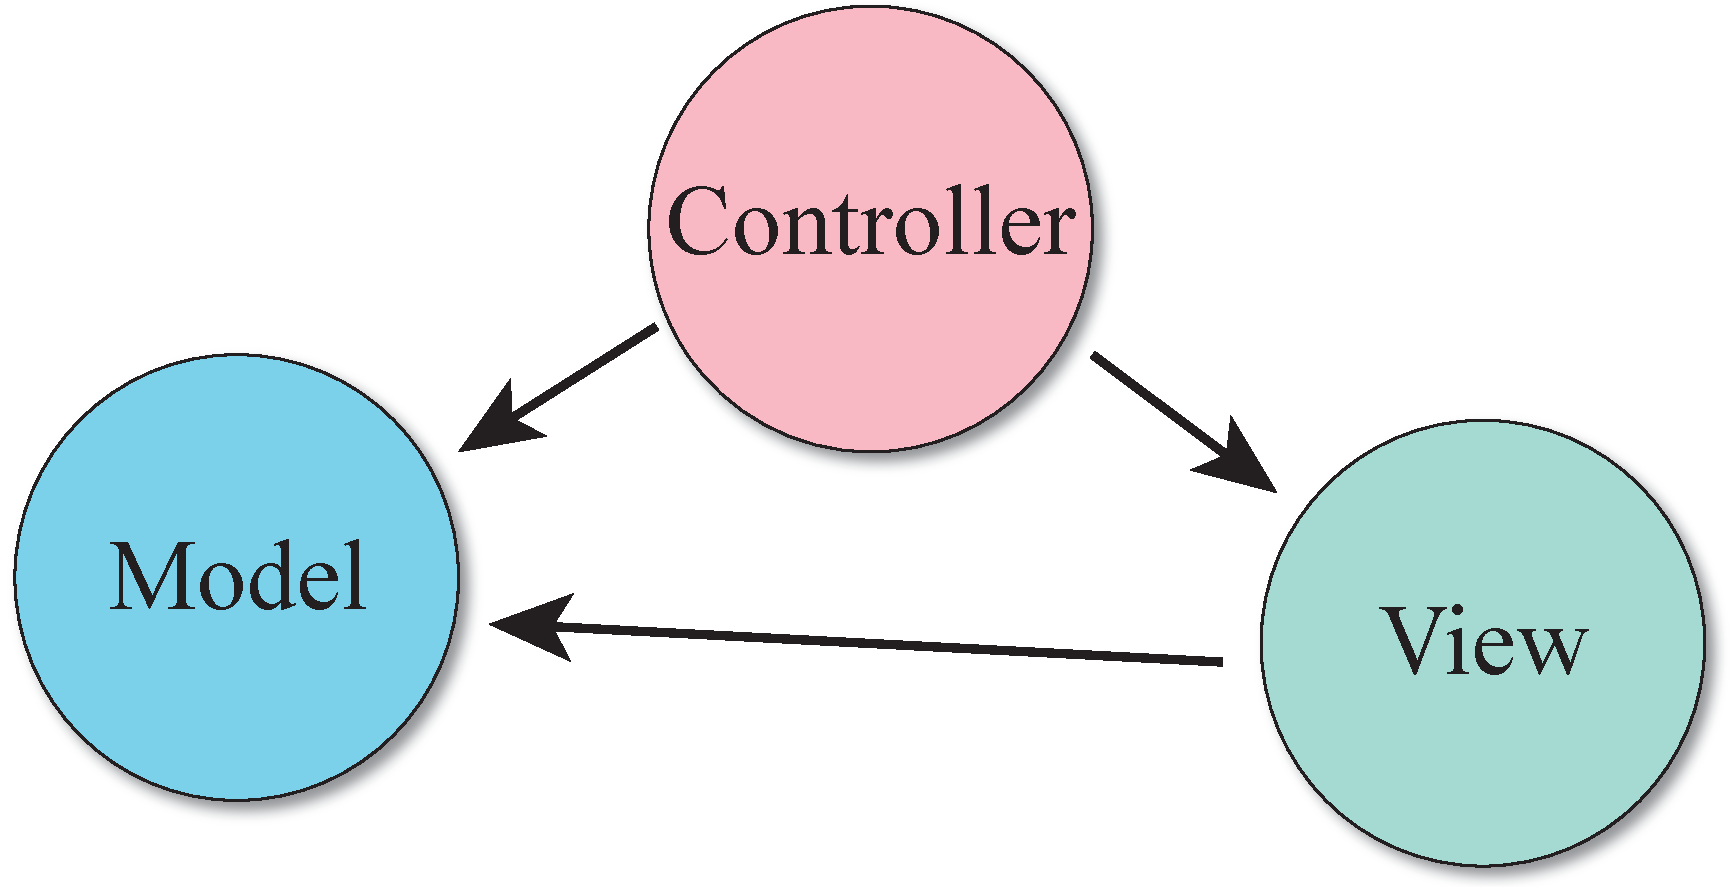
\includegraphics[width=10cm]{fig/mvc}
	\caption{Direkte Assoziationen zwischen Model, View und Controller}
\end{figure}

\paragraph{Model:}
Verantwortlich für alles, was die Daten eines bestimmten Models angeht. In der Anwendung ist dieser Bereich für Interaktionen, Gültigkeit und Auswertung verantwortlich und repräsentiert hier zum Beispiel eine Veranstaltung, einen Benutzer, Statistiken oder Koordinaten der Benutzer.

\paragraph{View:}
Generiert das Aussehen einer bestimmten Seite. Hier wird vorwiegend mit gängigen Webformaten, wie HTML, PHP und JavaScript gearbeitet. Ein View kann auf die Daten zugreifen, die ihm der Controller liefert und diese dann anschaulich darstellen. Dadurch muss sich ein View nicht darum kümmern, woher er seine Informationen zusammensuchen muss, sondern bekommt garantiert, dass diese vom Controller bereitgestellt werden. Auf diese Weise können verschiedene Views für verschiedene Geräte erstellt werden und erlauben einfach eine mobile Seite zu generieren.

\paragraph{Controller:}
Hier findet die gesamte Logik und Aufbereitung der Daten statt, die später dem Benutzer im View angezeigt werden sollen. Sämtliche Datenbankabfragen, Berechnungen oder Ähnliches werden hier durchgeführt und dem Model / View bereitgestellt. Für jedes Objekt existiert ein eigener Controller. Diese werden \emph{EventsController}, \emph{UsersController} etc. genannt.\\
In diesem Framework ist jede Methode direkt mit den Views verknüpft, das heißt definiert man im EventsController eine Funktion namens \emph{index()}, so stellt dies eine Seite der Webanwendung dar, die mit \emph{http://localhost/Events/index} aufgerufen werden kann und den entsprechenden View in \emph{/View/Events/index.ctp} erwartet.\par

Die Vorteile bei diesem Entwurfsmuster liegen auf der Hand: Es muss nur einmal ein Objekt im Model definiert werden. Im Controller wird die komplette Logik verarbeitet und damit kann man mit entsprechenden Views für verschiedene Ansichten (z.B. eine mobile Anwendung der App) einfach auf die Daten des Controllers zugreifen. Der Code kann dadurch kompakter gehalten werden und muss nur im Controller angepasst werden, um auf allen Ansichten der Seite die Daten aktualisieren zu können.

%%%%%%%%%%%%%%%%%%%%%%%%%%%%%%%%%%%%%%%%%%%%%%%%%%%%%%%%%%%%%%%%%%%%%%%%%%%%%%%%%%%%%%%%%%%%%%%%%%%%%%%%%%%%%%%%%%%%%%%%%%%%%%

\section{Datenbanken}
Um alle Daten schnell und einfach verarbeiten zu können, ist eine Datenbank nötig. Da es sich hier um eine Webanwendung handelt, bietet sich eine SQL Datenbank an, weil diese in der Regel zum Komplettpaket eines Webservers gehört.\\
Folgende Tabellen wurden angelegt:

\paragraph{users:}
Ein Benutzer besteht aus einer eindeutigen Identifizierungsnummer (\emph{ID}), einem Benutzernamen, einem Passwort und einer zugewiesenen Rolle (z.B. Administrator, Benutzer usw.). Dazu werden von der App automatisch zwei Zeitstempel mit Erstellungs- und letztem Änderungsdatum sowie einem Boolean hinzugefügt, welcher angibt, ob der Benutzer sich im System der Webanwendung einloggen kann und damit Daten einsehen kann.

\paragraph{events:}
Verpflichtende Felder sind ein Titel und eine Beschreibung. Dazu wird von der App eine eindeutige ID zugewiesen und die Benutzer-ID des Benutzers hinzugefügt, welcher diese Veranstaltung erstellt. Dazu noch zwei Zeitstempel: Erstellungsdatum und Zeitpunkt der letzten Änderung.\par

Dies sind die beiden grundlegenden Tabellen, die für diese Anwendung nötig sind. Jedoch besteht noch keine Verknüpfung untereinander, abgesehen von der Benutzer-ID in der \emph{events}-Tabelle.

\subsection{Verknüpfung von Benutzer und Veranstaltung}
Um einer Veranstaltung beliebig viele Benutzer zuordnen zu können, wurde die Tabelle \emph{events\_users} erstellt. Diese beinhaltet nur die Fremdschlüssel ID aus den \emph{events}- und \emph{users}-Tabellen.

\begin{figure}[!ht]
	\centering
	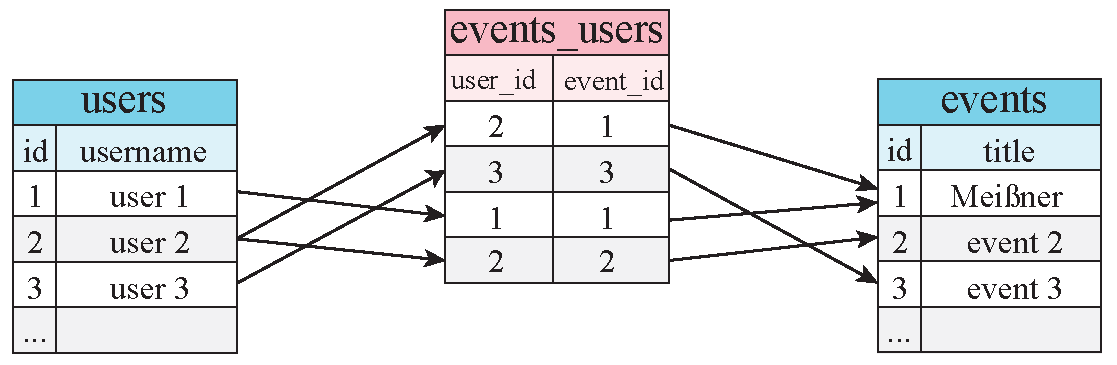
\includegraphics[width=15cm]{fig/events_users}
	\caption[Zuweisung eines Benutzers zu einer Veranstaltung]{Zuweisung eines Benutzers zu einer Veranstaltung (vereinfacht)}
\end{figure}

Diese \emph{Many-to-many}-Verknüpfung (in cakePHP auch \emph{hasAndBelongsToMany, HABTM} genannt) kann der EventsController mit einer einzigen SQL-Abfrage erfragen und erhält damit alle dem Event zugeordneten Benutzer. Diese Daten können dann in einer Variable gespeichert und dem View bereitgestellt werden.

\subsection{Veranstaltungsspezifische Eigenschaften}
Die ersten Schritte zu einer Webanwendung, die Veranstaltungen und Benutzer verwalten kann, sind nun erledigt. Bisher ist es allerdings nicht möglich in Veranstaltungen Felder zu definieren, die für eben jene Veranstaltung von Bedeutung sind. Das können im konkreten Fall Felder sein wie \glqq Art des Transportmittels\grqq{}, \glqq Wird ein Parkplatz benötigt?\grqq{}, \glqq Welcher Holzstangenbedarf besteht?\grqq{} oder Ähnliches.

\paragraph{Key-Value-Store} In einem Key-Value-Store wird die Datenbank mit den Werten (\emph{values}) über die Schlüssel (\emph{keys}) indexiert. Der Vorteil ist, dass vorher nicht bekannt sein muss, welche Werte in die Datenbank eingetragen werden sollen.\\
In der Meißner App wurde diese Methode implementiert, um eventspezifisch ein beliebiges Feld zu definieren, welches Werte als Strings annimmt. So ist gewährleistet, dass die Benutzer dieser Anwendung die größtmögliche Freiheit besitzen, was die Inhalte der Veranstaltungen angeht. Jede kann individuell angelegt und personalisiert werden, sodass sie den gewünschten Anforderungen genügt.\\
Um die häufigsten Nutzungsszenarien abzudecken, wurden Strings als Hauptformat für die Values gewählt. Diese lassen sich einfach auswerten und erhalten die einfache Bedienung der Formulare.\\
Für die automatischen Statistiken ist das Format irrelevant, da nur auf Gleichheit der Strings geprüft wird und anhand dessen die Grafiken erstellt werden. 

\paragraph{Implementierung}
Für die Implementierung sind zwei weitere Tabellen notwendig: 

\begin{enumerate} 
	\item \emph{event\_columns}: Dient als Maske, um Feldnamen und -typen zu definieren. Kann zudem innerhalb einer speziellen Veranstaltung genutzt werden, um diese Felder den zugeordneten Benutzern verfügbar zu machen.
	\item \emph{event\_properties}: Im View wird ein Formular generiert, welches die Feldnamen aus \emph{event\_columns} anzeigt und die Möglichkeit gibt, Werte einzutragen. Diese Werte werden dann über den Controller in \emph{event\_properties} gespeichert.
\end{enumerate}

Mit den Tabellen steht nun die Datenstruktur zur Verfügung, die es ermöglicht verantstaltungsspezifische Eigenschaften zu erstellen und die so erzeugten Felder mit den entsprechenden Werten der Teilnehmer dieser Veranstaltung zu befüllen.

\begin{figure}[!ht]
	\centering
	\includegraphics[width=15cm]{fig/event_properties}
	\caption[Speichern von spez. Feldern in die Datenbank]{Controller erfragt Felder aus event\_columns, stellt sie dem View zur Verfügung, speichert danach die Werte in event\_properties}
\end{figure}

Obige Abbildung zeigt kurz das Zusammenspiel von Controller und View: Datenbankzugriffe werden über den View an den Controller gerichtet und dort ausgeführt. So können Daten abgefragt oder neue Daten geschrieben werden.\par

Als einzigartige primäre Schlüssel werden \emph{user\_id} und \emph{key} gewählt, womit automatisch Duplikate ausgeschlossen werden. Somit kann immer nur genau ein Wert in einem benutzerspezifischen Feld des Benutzers stehen.\\
Beispiel: In der Abbildung existiert die Zeile \emph{Benutzer: 42, Event: 3, Key: gender, Value: male}. Wenn der Benutzer nun das Geschlecht in dem Formular ändert und das abschickt, dann sieht die Nachricht so aus: \emph{Benutzer: 42, Event: 3, Key: gender, Value: female}. Weil das Feld \emph{key} als Primärschlüssel definiert wurde, wird dieser Eintrag überschrieben und kein neuer Eintrag in der Datenbank angelegt.

\section{Verhinderung von Angriffen}
Gängige Angriffsmethoden, wie Cross-Site-Scripting oder SQL-Injection, werden in dieser Arbeit weitgehend verhindert.

\subsection{SQL-Injection}
Bei der \emph{SQL-Injection} versucht ein Angreifer durch geschicktes Manipulieren von Eingabefeldern eines Formulars, einen String zu erzeugen, mit dem er einen ungewollten Zugang zur Datenbank erhält. Schafft er das, so kann er Datensätze aus der SQL Tabelle ausgeben lassen, verändern oder sogar komplett löschen.\par

Um diese Art der Angriffe zu verhindern, haben die Entwickler von cakePHP einige Sicherheitsvorkehrungen implementiert. Zusätzlich gibt es das Modul \emph{Sanitize}, welches die Eingabestrings des Benutzers überprüft und alle Sonderzeichen, wie Hochkommata und Semikolons, aus dem String entfernt. Damit lässt sich keine zusätzliche Anweisung in den SQL-Query mit einbauen und die Anwendung ist somit weitgehend vor diesen Angriffen geschützt.

\subsection{Cross-Site-Scripting XSS}
Mit \emph{XSS} beschreibt man eine Angriffsmethode, die webseitenübergreifend Schadcode über normale Hyperlinks ausführt. Dabei können bei Clients, die JavaScript unterstützen, Cookies an den Angreifer übertragen werden.\par

Auch hier übernimmt cakePHP das Abwehren dieser Angriffe. Damit diese Mechanismen auch greifen, werden in dieser Webanwendung die von den Entwicklern vorgeschlagenen Paradigmen beachtet.

%%%%%%%%%%%%%%%%%%%%%%%%%%%%%%%%%%%%%%%%%%%%%%%%%%%%%%%%%%%%%%%%%%%%%%%%%%%%%%%%%%%%%%%%%%%%%%%%%%%%%%%%%%%%%%%%%%%%%%%%%%%%%%

\section{Views entwickeln}
Nun wurde mit modernen Webtechnologien und möglichst geringem Aufwand direkt eine mobile Seite der Anwendung erstellt, welche für Smartphone und Tablets optimiert ist. Schließlich soll und muss diese Web-App auch auf dem Gelände mobil genutzt werden können.\par

Dabei gibt es mehrere Ansätze, wobei in dieser Arbeit das sogenannte \emph{Responsive Webdesign} (deutsch: bedarfsgesteuertes Webdesign) für die mobile Version der Anwendung benutzt wird.

\subsection{Responsive Webdesign mit jQuery Mobile}
Hauptaugenmerk wird hier auf die Auflösung des Endgeräts gelegt: Handelt es sich hierbei um ein günstiges Smartphone mit schlechtem Display, um ein Google Nexus 10 mit 2560x1600 Pixeln oder um einen SmartTV mit FullHD?\\
Diese Frage ist entscheidend, denn sie bestimmt wie viele und wie groß bestimmte Objekte im Sichtbereich des Geräts sein können, sodass der Benutzer nicht von der schlechten Bedienung genervt ist, sondern weiterhin die Informationen aus der App holen möchte. Beim Responsive Webdesign werden über \emph{Media Queries} (Abfrage der Eigenschaften des Geräts, Beispiel: Auflösung, Orientierung des Endgeräts usw.) Informationen des Endgeräts eingeholt und darauf abgestimmte Stylesheets geladen.\par

Um aber eine Webanwendung zu entwickeln, die aussieht und sich \glqq anfühlt\grqq{} wie eine echte App wurde in dieser Arbeit das Framework \emph{jQuery Mobile} verwendet, welches auch auf Responsive Webdesign setzt und dabei viele Steuerelemente zur Verfügung stellt, die dem Benutzer schon von nativen Apps her bekannt sind, wie typische Slider, Buttons, Dropdown-Menüs und vielem mehr.

\newpage
\paragraph{Mobile View}
Damit jQuery Mobile aus normalen Links touchoptimierte Bedienelemente erzeugt, konnte nahezu der komplette Code von der Desktop-Version genommen werden. Lediglich kleine Ergänzungen um das \emph{data-role} Attribut sind notwendig, damit jQuery Mobile diese anpassen kann, das bedeutet ein normaler Hyperlink wird um \emph{data-role="button"} erweitert.\\

\begin{lstlisting}[captionpos=b, caption=Eine kleine Ergänzung erzeugt aus einem Link einen touchfreundlichen Button]
  <a href="#">normal link</a>
  <a href="#" data-role="button">touchoptimized link</a>
\end{lstlisting}

Auf ähnliche Art und Weise können auch viele andere Elemente umgewandelt werden, damit diese für Smartphones optimiert sind. Oft erfolgt dies automatisch, da jQuery Mobile Bedienelemente erkennt und diese dann sofort anpasst.


\chapter{Echtzeitaktualisierung mit WebSockets}
Mit der Echtzeitaktualisierung wird ein zeitlich direkter Datenaustausch zwischen Endgeräten über einen separaten WebSocket Server (kurz: WS Server) ermöglicht. 

\section{Einführung in WebSockets}
Mit der HTML5-Spezifikation wurden \emph{WebSockets}, ein auf \emph{TCP} basierendes Protokoll der Anwendungsschicht, eingeführt, welches eine Vollduplex, bidirektionale, Single-Socket Verbindung ermöglicht \cite[S. 7]{ws}. Eine Anfrage öffnet die Verbindung zum WebSocket Server und kann beliebig lange offen gehalten werden, wobei zu jeder Zeit Daten zwischen Client und Server ausgetauscht werden. Dieser Datenaustausch geschieht sehr schnell und mit einem sehr kleinen Overhead, da die Verbindung nicht neu aufgebaut werden muss und die Daten somit sofort verschickt werden können.\\
Ähnlich wie \glqq normale\grqq{} Sockets werden WebSockets von einer Anwendung erzeugt und stellen dann die Schnittstelle zwischen der Webanwendung und dem Transportprotokoll TCP dar.\\
Im direkten Vergleich zu den generischen Sockets, erfüllen WebSockets eine ähnliche Funktion, sind allerdings auf Webanwendungen und TCP beschränkt. 

\paragraph{Handshake} 
Der Handshake erfolgt über HTTP/1.1 und ähnelt dem zum Aufruf einer Homepage:
\\
\begin{lstlisting}[captionpos=b, caption=HTTP Request des Clients {\cite[S. 6]{rfc6455:handshake}}]
  GET / HTTP/1.1
  Host: server.example.com
  Origin: http://www.example.com
  Sec-WebSocket-Key: 7+C600xYyb0v2zmJ69RQsw==
  Sec-WebSocket-Version: 13
  Upgrade: WebSocket
\end{lstlisting}

Mit \emph{Upgrade: WebSocket} wird signalisiert, dass der Client eine WebSocket-Verbindung zum Server aufbauen möchte. Der entsprechende WS Server reagiert darauf mit dem HTTP-Statuscode \emph{101 Switching Protocols}, womit er bestätigt, dass er mit dem Wechsel des Protokolls einverstanden ist.
\\
\begin{lstlisting}[captionpos=b, caption=HTTP Response des Servers {\cite[S. 8]{rfc6455:handshake}}]
  101 Switching Protocols
  Connection: Upgrade
  Sec-WebSocket-Accept: fYoqiH14DgI+5y1EMwM2sOLzOi0=
  Upgrade: WebSocket
\end{lstlisting}

Der kryptische Schlüssel \emph{Sec-WebSocket-Accept} muss vom Server berechnet und zurückgegeben werden und zeigt damit, dass er das WebSocket Protokoll versteht. Ab diesem Zeitpunkt ist der Handshake abgeschlossen und die Verbindung wurde aufgebaut.\par

\begin{figure}[!ht]
	\centering
	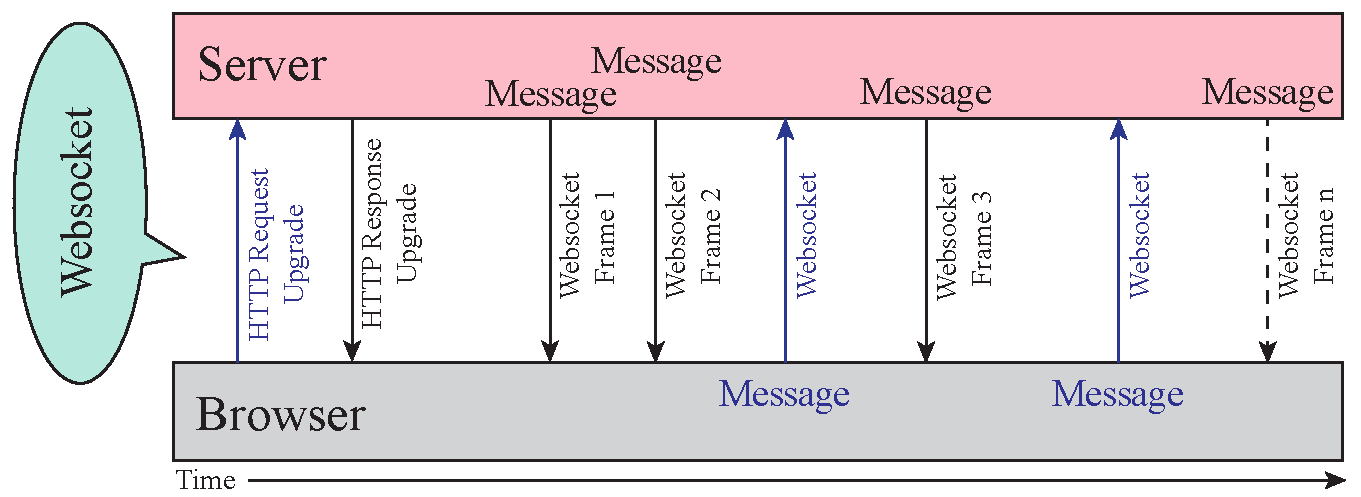
\includegraphics[width=15cm]{fig/websockets}
	\caption[Aufbau einer WebSocket Verbindung]{Aufbau einer WebSocket Verbindung. Danach können beliebig Nachrichten in beide Richtungen (gleichzeitig) übermittelt werden {\cite[S. 7]{ws}}}
\end{figure}

Nun kommen die Vorteile von WebSockets zur Geltung: nach erstmaligem Aufbau der Verbindung bleibt diese geöffnet und zu jedem Zeitpunkt können Client und Server die Vollduplex Verbindung nutzen, um Daten miteinander auszutauschen. So kann ein fast volles TCP innerhalb einer Webanwendung verwendet werden.\\
Es verringern sich außerdem die Latenzzeiten, der Traffic und die CPU-Leistung der Server. Das liegt daran, dass die Pakete direkt zugestellt werden können, der Overhead dank einmaligem Handshake deutlich geringer ist und der Austausch der Daten sehr einfach gestaltet ist. 

%%%%%%%%%%%%%%%%%%%%%%%%%%%%%%%%%%%%%%%%%%%%%%%%%%%%%%%%%%%%%%%%%%%%%%%%%%%%%%%%%%%%%%%%%

\section{Implementierung der Echtzeitaktualisierung}
Im ersten Ansatz dieser Arbeit wurde der WebSocket-Server auf Basis von \emph{node.js} \cite{node.js}, einem serverseitigem JavaScript Framework für Server, implementiert. Das verlief aufgrund der einfachen Handhabung von WebSockets und der guten Unterstützung von HTML5 problemlos. Jedoch wurden zu diesem Zeitpunkt weder verschlüsselte Verbindungen noch Broadcasting unterstützt. Daher war dies ungeeignet, weil sensible Daten, wie die Standorte der Clients, nicht im Klartext verschickt werden sollten.\\
Außerdem ist eine Broadcast-Funktion notwendig, die den bestehenden Sockets bei Aktualisierung einer Position sofort die neuen Koordinaten übermittelt.\par

Die Implementierung beider Funktionen hätte den Rahmen dieser Arbeit überschritten, weshalb serverseitig das Open Source Framework \emph{socket.io} für node.js verwendet wird. Es stellt sämtliche benötigten Dienste sowie einen Fallback bereit, wodurch auch älteren Browsern ohne HTML5 Unterstützung eine websocketähnliche Verbindung ermöglicht wird.\par

Clientseitig wurde ein Skript in JavaScript entwickelt, welche im Hintergrund der Web-App ausgeführt wird. Es verbindet sich mit dem WebSocket Server, schickt initial die aktuellen Koordinaten unabhängig davon, welcher View gerade angezeigt wird und wartet auf eingehende Nachrichten oder auf eine Änderung der eigenen Position. Bewegt sich der Client, werden automatisch die Koordinaten GoogleMaps-kompatibel in Form von Latitude und Longitude an den WebSocket Server übermittelt.\\
Erhält der Server so eine Nachricht, aktualisiert er seine Datenbank von Standorten der Clients und schickt per Broadcast eine Nachricht an alle verbundenen Clients. So erhalten die Endgeräte in Echtzeit eine Aktualisierung aller Positionen.

\paragraph{Fallback}
Nicht jedes Endgerät unterstützt die Verwendung von WebSockets. Zwar gab es keine Komplikationen mit den getesteten Geräten, da WebSockets mit allen gängigen Desktop Browsern und fast allen mobilen Browsern außer Opera Mini lauffähig ist. Bei veralteter Software ist eine eine Unterstützung jedoch nicht immer gegeben. Daher wurde socket.io so eingerichtet, dass ein Fallback über \emph{flashsockets} hin zum \emph{polling} ermöglicht wird. So kann der größte Teil aller Browser die Echtzeitaktualisierung verwenden.

\paragraph{Entwicklung eines eigenen Protokolls zur Kommunikation über WebSockets}
Um bestimmte Funktionen auf dem Server anzusprechen, wurde ein einfaches Protokoll entwickelt, welches angibt, um welchen Inhalt es sich bei der Nachricht handelt. Alle Nachrichten, die zwischen Client und Server ausgetauscht werden, werden vorher intern als JSON Objekte benutzt und für die Übertragung über die WebSockets in Strings konvertiert. Dabei enthalten alle Nachrichten ein Feld \emph{type}, welches folgende Werte annehmen kann:

\begin{itemize}
	\item[] \emph{location:} enthält Latitude und Longitude des Clients
	\item[] \emph{syn:} enthält eine Signatur für die Authentifizierung
	\item[] \emph{subscribe:} abonniert bestimmte Events, dazu später mehr
	\item[] \emph{publish:} signalisiert eine Änderung an der Datenbank
	\item[] \emph{message:} eine neue Chat Nachricht hat den Server erreicht und wird per Broadcast an die Clients verschickt
	\item[] \emph{history:} Anfrage eines Clients nach der aktuellen Historie des Chats
\end{itemize}

Der socket.io Server wertet diese Fälle über ein \emph{Switch-Case-Statement} aus und ruft entsprechende Methoden zur weiteren Verarbeitung auf.

%%%%%%%%%%%%%%%%%%%%%%%%%%%%%%%%%%%%%%%%%%%%%%%%%%%%%%%%%%%%%%%%%%%%%%%%%%%%%%%%%%%%%%%%%

\section{Kommunikation zwischen Apache und WebSocket Server}
Bei dem Webserver Apache und dem WebSocket Server mit dem Framework socket.io handelt es sich um zwei Anwendungen, die selbstständig und unabhängig voneinander aktiv sind. Beide verwenden HTTP und werden mit HTTP Requests angesprochen. Diese Implementierung sieht vor, dass beide parallel auf einem Server ausgeführt und mit verschiedenen Ports angesprochen werden.\\
Um die Berechtigungen des WebSocket Servers möglichst gering zu halten und diesen nur für die Echtzeitaktualisierung zu nutzen, hat socket.io keinerlei Rechte, um auf die Datenbank oder andere Elemente der Webanwendung zugreifen zu können. Dadurch bleibt die Kapselung beider Anwendungen erhalten, aber ein weiterer Schritt zur Authentifizierung eines Benutzers ist erforderlich.

\paragraph{WebSockets über PHP mit ElephantIO}
Damit die Meißner App selbst eine Verbindung zum WebSocket Server aufbauen kann, ist die Open Source Bibliothek \emph{ElephantIO} \cite{elephant.io} erforderlich. Sie ermöglicht die Kommunikation mit Apache und socket.io, da diese sonst nicht ohne Weiteres möglich ist. So gibt es die Funktion, dass die Webanwendung selbst Nachrichten an den WS Server schicken kann.\\
Die Kommunikation in die andere Richtung ist nicht notwendig, da die Web-App keine Informationen benötigt welche Endgeräte sich über WebSockets angemeldet haben.

%%%%%%%%%%%%%%%%%%%%%%%%%%%%%%%%%%%%%%%%%%%%%%%%%%%%%%%%%%%%%%%%%%%%%%%%%%%%%%%%%%%%%%%%%

\section{Authentifizierung eines Clients beim WebSocket Server}
In der Webanwendung kann mit einem normalen Formular der Benutzername und das Passwort eingegeben werden, allerdings hat der WS Server bekanntlich keinen Zugang zur Datenbank. Es muss aber eine Authentifizierung am WebSocket Server stattfinden, damit nur Benutzer aus der Webanwendung eine Verbindung erstellen können. Dafür wird das \emph{RSA Kryptosystem} verwendet.

\paragraph{Erzeugung der Schlüssel}
Zur ersten Initialisierung der Webanwendung erstellt die Webanwendung sich selbst per RSA-Verfahren einen 2048-Bit langen privaten und einen öffentlichen Schlüssel. Sie gehören ausschließlich der Meißner App selbst und werden lokal gespeichert. Der öffentliche Schlüssel wird dem WebSocket Server bereitgestellt, welcher sich diesen direkt aus dem entsprechenden Ordner in der Webanwendung laden kann. Das ist sinnvoll, weil WS Server und Webanwendung sich vertrauen können, da sie auf der gleichen Maschine laufen.

\paragraph{Signieren der Nachricht und anschließende Authentifizierung}
Wenn sich nun ein Client in der Webanwendung mit Benutzernamen und Passwort erfolgreich einloggt, nimmt die App den Benutzernamen $user$ und erstellt mit dem privaten Schlüssel eine Signatur $sig = sign(user)$, welche dem Client zur Verfügung gestellt wird. Damit kann dieser nun einen syn-Request mit Benutzernamen und Signatur an den WebSocket Server schicken. Dieser überprüft nun die Signatur mit dem öffentlichen Schlüssel $verify(sig)$ und wenn diese der ursprünglichen Nachricht entspricht, ist der Client authentifiziert.

\begin{figure}[!ht]
	\centering
	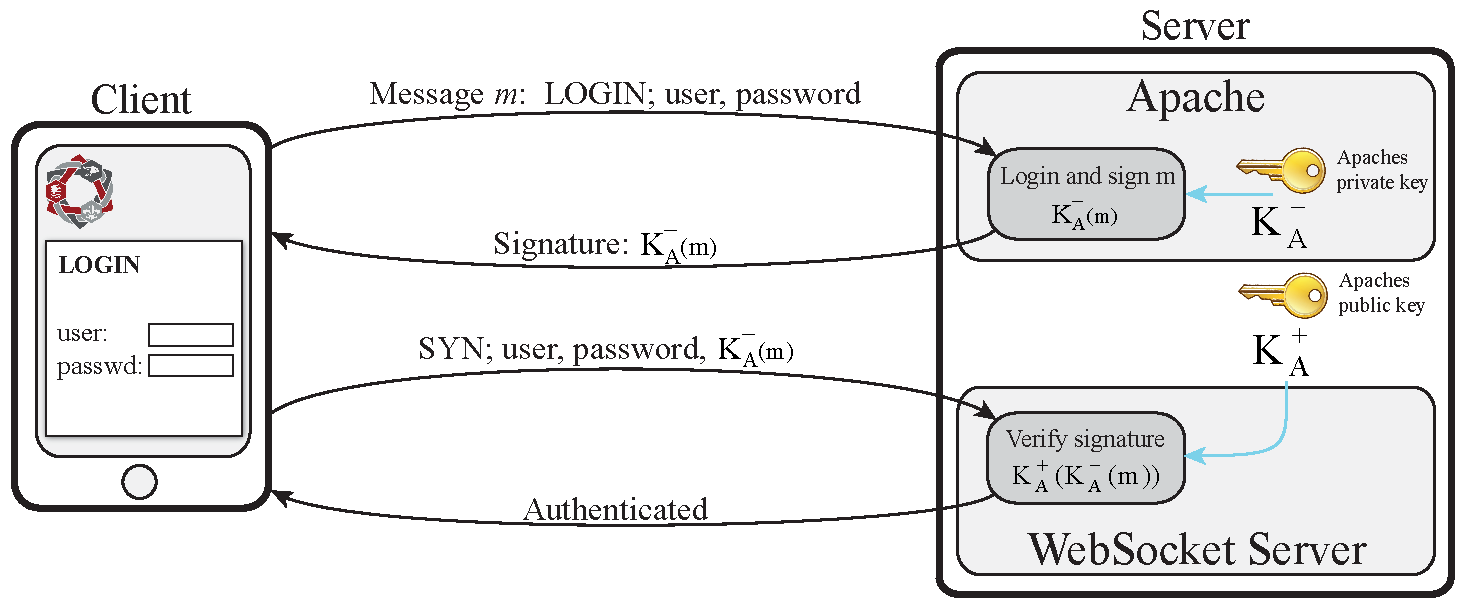
\includegraphics[width=15cm]{fig/publicprivate}
	\caption{Authentifizierung eines Clients beim Server}
\end{figure}

\paragraph{Vorteile dieser Implementierung}
Durch diese Authentifizierung kann socket.io alle eingehenden Verbindungen ablehnen, die keine korrekte Signatur erhalten haben. Ein Angreifer muss somit über den Benutzernamen und das Passwort eines Benutzers verfügen, um sowohl zu der Webanwendung als auch zum WS Server einen Zugang zu erhalten. Er kann nun aber nicht ohne diese Daten eine Verbindung aufbauen und Daten abgreifen.\par

Dieser Weg der Authentifizierung wurde gewählt, da zum Zeitpunkt des Logins der WebSocket des Endgeräts noch nicht bekannt ist. Also kann die Webanwendung dem WS Server nicht mitteilen, welcher Benutzer zu welchem WebSocket gehört. Ein zweiter Schritt zur endgültigen Authentifizierung über eine Signatur ist also notwendig für die korrekte Zuordnung vom offenen WebSocket zum Benutzer. 

%%%%%%%%%%%%%%%%%%%%%%%%%%%%%%%%%%%%%%%%%%%%%%%%%%%%%%%%%%%%%%%%%%%%%%%%%%%%%%%%%%%%%%%%%

\section{Entwurfsmuster: Publish / Subscribe}
Mit Publish / Subscribe (deutsch: veröffentlichen / abonnieren) wird ein Muster beschrieben, mit dem ein Client eine Benachrichtigung erhält, sofern ein Ereignis verändert wurde, welches von ihm abonniert wurde. Bei diesem Entwurfsmuster wissen weder Publisher noch Subscriber voneinander und es läuft vollkommen unabhängig, asynchron miteinander. Sie müssen auch nichts voneinander wissen, da sämtlicher Datenaustausch über den socket.io Server läuft \cite{autobahn.js:pubsub}.\par

Konkret können in dieser Anwendung Veranstaltungen abonniert werden. Das geschieht automatisch über die Webanwendung selbst, welche dem WebSocket Server mit Einloggen des Benutzers eine subscribe Nachricht schickt. Ausgewählt werden die Events, die der Benutzer selbst erstellt hat. 

Gab es eine Änderung an einer Veranstaltung, so meldet sich die Web-App beim WebSocket Server mit einer \emph{publish}-Nachricht. Dieser schaut dann in seiner Liste der authentifizierten Clients nach, welcher die Veranstaltung abonniert hat und schickt an alle verbundenen Endgeräte eine Mitteilung, dass die Veranstaltung bearbeitet wurde.\par

\paragraph{Implementierung}
Im ersten Entwurf der Technik in dieser Arbeit wurden alle Nachrichten, die über WebSockets verschickt wurden, über die Clients selbst versendet, da die Kommunikation nur über JavaScript nativ unterstützt wird. Daher wurden auf Basis von Elephant.io Methoden entwickelt, die die publish-Funktion der Webanwendung übernehmen.\\
Der EventsController hat nun noch die zusätzliche Aufgabe bei jedem Datenbankzugriff eine Verbindung zum WS Server zu öffnen, eine publish-Nachricht abzuschicken, und dann die Verbindung wieder zu schließen.\\
Dadurch funktioniert Publish/Subscribe auch mit Endgeräten, die JavaScript verbieten. Die Clients, die Nachrichten erhalten möchten, bekommen diese nun ungehindert zugestellt.\par

\begin{figure}[!ht]
	\centering
	\includegraphics[width=15cm]{fig/noty_android}
	\caption{publish-Benachrichtigung am unteren Bildschirmrand mit Android 4.3}
\end{figure}

So ist es nun möglich über WebSockets eine Benachrichtigung an die Abonnenten zu schicken. Dadurch wird man aktiv informiert, wenn Änderungen an den Veranstaltungen vorgenommen werden. 

%%%%%%%%%%%%%%%%%%%%%%%%%%%%%%%%%%%%%%%%%%%%%%%%%%

\section{Vor HTML5: Benutzung von Polling}
Für den Datenverkehr von Internetseiten wird bekanntlich HTTP benutzt, welches die wechselseitige Datenübermittlung \emph{Halbduplex} verwendet. So erfolgt der Datenverkehr nur in eine Richtung zur gleichen Zeit: der Client schickt eine Anfrage an den Server und dieser übermittelt danach die Antwort \cite[S. 5]{ws}. Das hat wiederum zur Folge, dass es relativ ineffizient ist, da man mit jeder Anfrage stets die Antwort des Servers abwarten muss.\par

\begin{figure}[!ht]
	\centering
	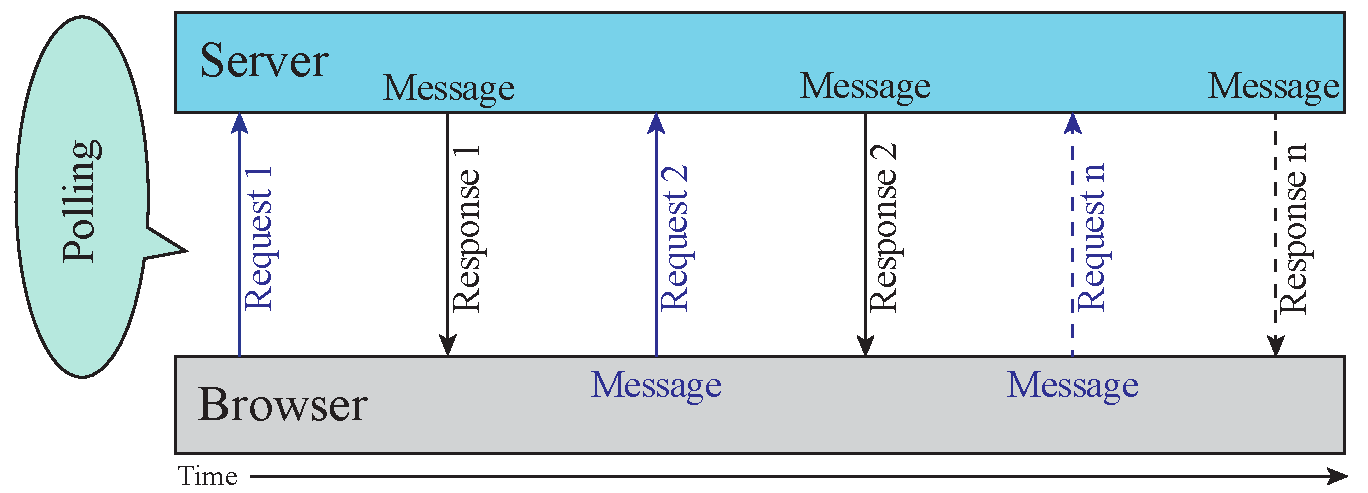
\includegraphics[width=15cm]{fig/polling}
	\caption[Datenaustausch beim Polling]{Datenaustausch mittels HTTP Request / Response beim Polling {\cite[S. 7]{ws}}}
\end{figure}

Vor diesem technischen Hintergrund wurde \emph{Polling} entwickelt, bei dem in einem zeitlich bekannten Intervall eine Anfrage an den Server geschickt wird mit der Bitte um Aktualisierung. Diese Technik ist sehr attraktiv, wenn die zeitlichen Abstände der Aktualisierung der Daten bekannt ist, allerdings sind Echtzeitdaten schlecht vorhersehbar. Dadurch ist Polling nicht die richtige Wahl für dieses Projekt, weil es auf eine wirkliche Echtzeitaktualisierung ankommt.\par

Da bei sämtlichen Techniken, die dem echtzeitähnlichen Austausch von Daten dienen, höhere Latenzen, mehr Rechenleistung und ein komplizierterer Aufbau zu erwarten sind, ist HTML5 mit WebSockets auf dem aktuellen Stand der Dinge und kann vieles besser machen als seine Vorgänger, weshalb für diese Arbeit auch auf diese junge Technik zurückgegriffen wird. Pollingähnliche Verbindungen werden bei dieser Webanwendung nur angewendet, wenn HTML5 oder die WebSockets von dem verwendeten Browser nicht unterstützt werden. Tritt so ein Fallback ein, so ist zwar immer noch die Kommunikation mit dem WebSocket Server möglich, aber es sind höhere Latenzen und erhöhter Traffic zu erwarten.

\chapter{Erweiterte Funktionen}
In diesem Kapitel werden nun weitere Funktionen beschrieben, die über die Grundausstattung der Web-App und die WebSockets hinausgehen, um die Arbeit zu erweitern und produktiver zu gestalten. 

%%%%%%%%%%%%%%%%%%%%%%%%%%%%%%%%%%%%%%%%%%%%%%%%%%

\section{Entwurfsmuster: Publish / Subscribe}
Mit Publish / Subscribe (deutsch: veröffentlichen / abonnieren) wird ein Muster beschrieben, mit dem ein Client eine Benachrichtigung erhält, sofern ein Ereignis verändert wurde, welches von ihm abonniert wurde. Bei diesem Entwurfsmuster wissen weder Publisher noch Subscriber voneinander und es läuft vollkommen unabhängig, asynchron miteinander. Sie müssen auch nichts voneinander wissen, da sämtlicher Datenaustausch über den socket.io Server läuft \cite{autobahn.js:pubsub}.\par

Konkret können in dieser Anwendung Veranstaltungen abonniert werden. Das geschieht automatisch über die Webanwendung selbst, welche dem WebSocket Server mit Einloggen des Benutzers eine subscribe Nachricht schickt. Ausgewählt werden die Events, die der Benutzer selbst erstellt hat. 

Gab es eine Änderung an einer Veranstaltung, so meldet sich die Web-App beim WebSocket Server mit einer \emph{publish}-Nachricht. Dieser schaut dann in seiner Liste der authentifizierten Clients nach, welcher die Veranstaltung abonniert hat und schickt an alle verbundenen Endgeräte eine Mitteilung, dass die Veranstaltung bearbeitet wurde.\par

\paragraph{Implementierung}
Im ersten Entwurf der Technik in dieser Arbeit wurden alle Nachrichten, die über WebSockets verschickt wurden, über die Clients selbst versendet, da die Kommunikation nur über JavaScript nativ unterstützt wird. Daher wurden auf Basis von Elephant.io Methoden entwickelt, die die publish-Funktion der Webanwendung übernehmen.\\
Der EventsController hat nun noch die zusätzliche Aufgabe bei jedem Datenbankzugriff eine Verbindung zum WS Server zu öffnen, eine publish-Nachricht abzuschicken, und dann die Verbindung wieder zu schließen.\\
Dadurch funktioniert Publish/Subscribe auch mit Endgeräten, die JavaScript verbieten. Die Clients, die Nachrichten erhalten möchten, bekommen diese nun ungehindert zugestellt.\par

\begin{figure}[!ht]
	\centering
	\includegraphics[width=15cm]{fig/noty_android}
	\caption{publish-Benachrichtigung am unteren Bildschirmrand mit Android 4.3}
\end{figure}

So ist es nun möglich über WebSockets eine Benachrichtigung an die Abonnenten zu schicken. Dadurch wird man aktiv informiert, wenn Änderungen an den Veranstaltungen vorgenommen werden. 

%%%%%%%%%%%%%%%%%%%%%%%%%%%%%%%%%%%%%%%%%%%%%%%%%%

\section{Lokalisierung von Clients}
Mit HTML5 wurde die \emph{navigator.geolocation} Klasse in die JavaScript API eingebaut. Diese Klasse ermöglicht es einer Webanwendung die Position des Anwenders zu erhalten - aber nur, wenn der Anwender zustimmt. Das geschieht mittels in der Umgebung befindlichen W-Lan Netzwerke, der eigenen IP und wird dann mit einem Google Service abgeglichen. Verfügt das Gerät über GPS, so werden diese Daten auch berücksichtigt und ermöglichen eine genauere Ortung \cite[1. Absatz]{html5:geolocations}.

\paragraph{Koordinieren von Helfern}
Um die eingetragenen Helfer in dieser Webanwendung besser koordinieren zu können, wurde daher ein Skript implementiert, welches im Hintergrund der Web-App läuft und die aktuelle Position des Endgeräts über eine SSL verschlüsselte Verbindung an den Server übermittelt. Unter der Voraussetzung, dass der Client diesem Vorgang zustimmt sind dem Server damit die Positionen der eingeloggten Benutzer bekannt. Diese Positionsdaten können dann von der Anwendung ausgewertet und in einer Karte von \emph{Google Maps} \cite{google:maps} visualisiert werden.

\begin{figure}[!ht]
	\centering
	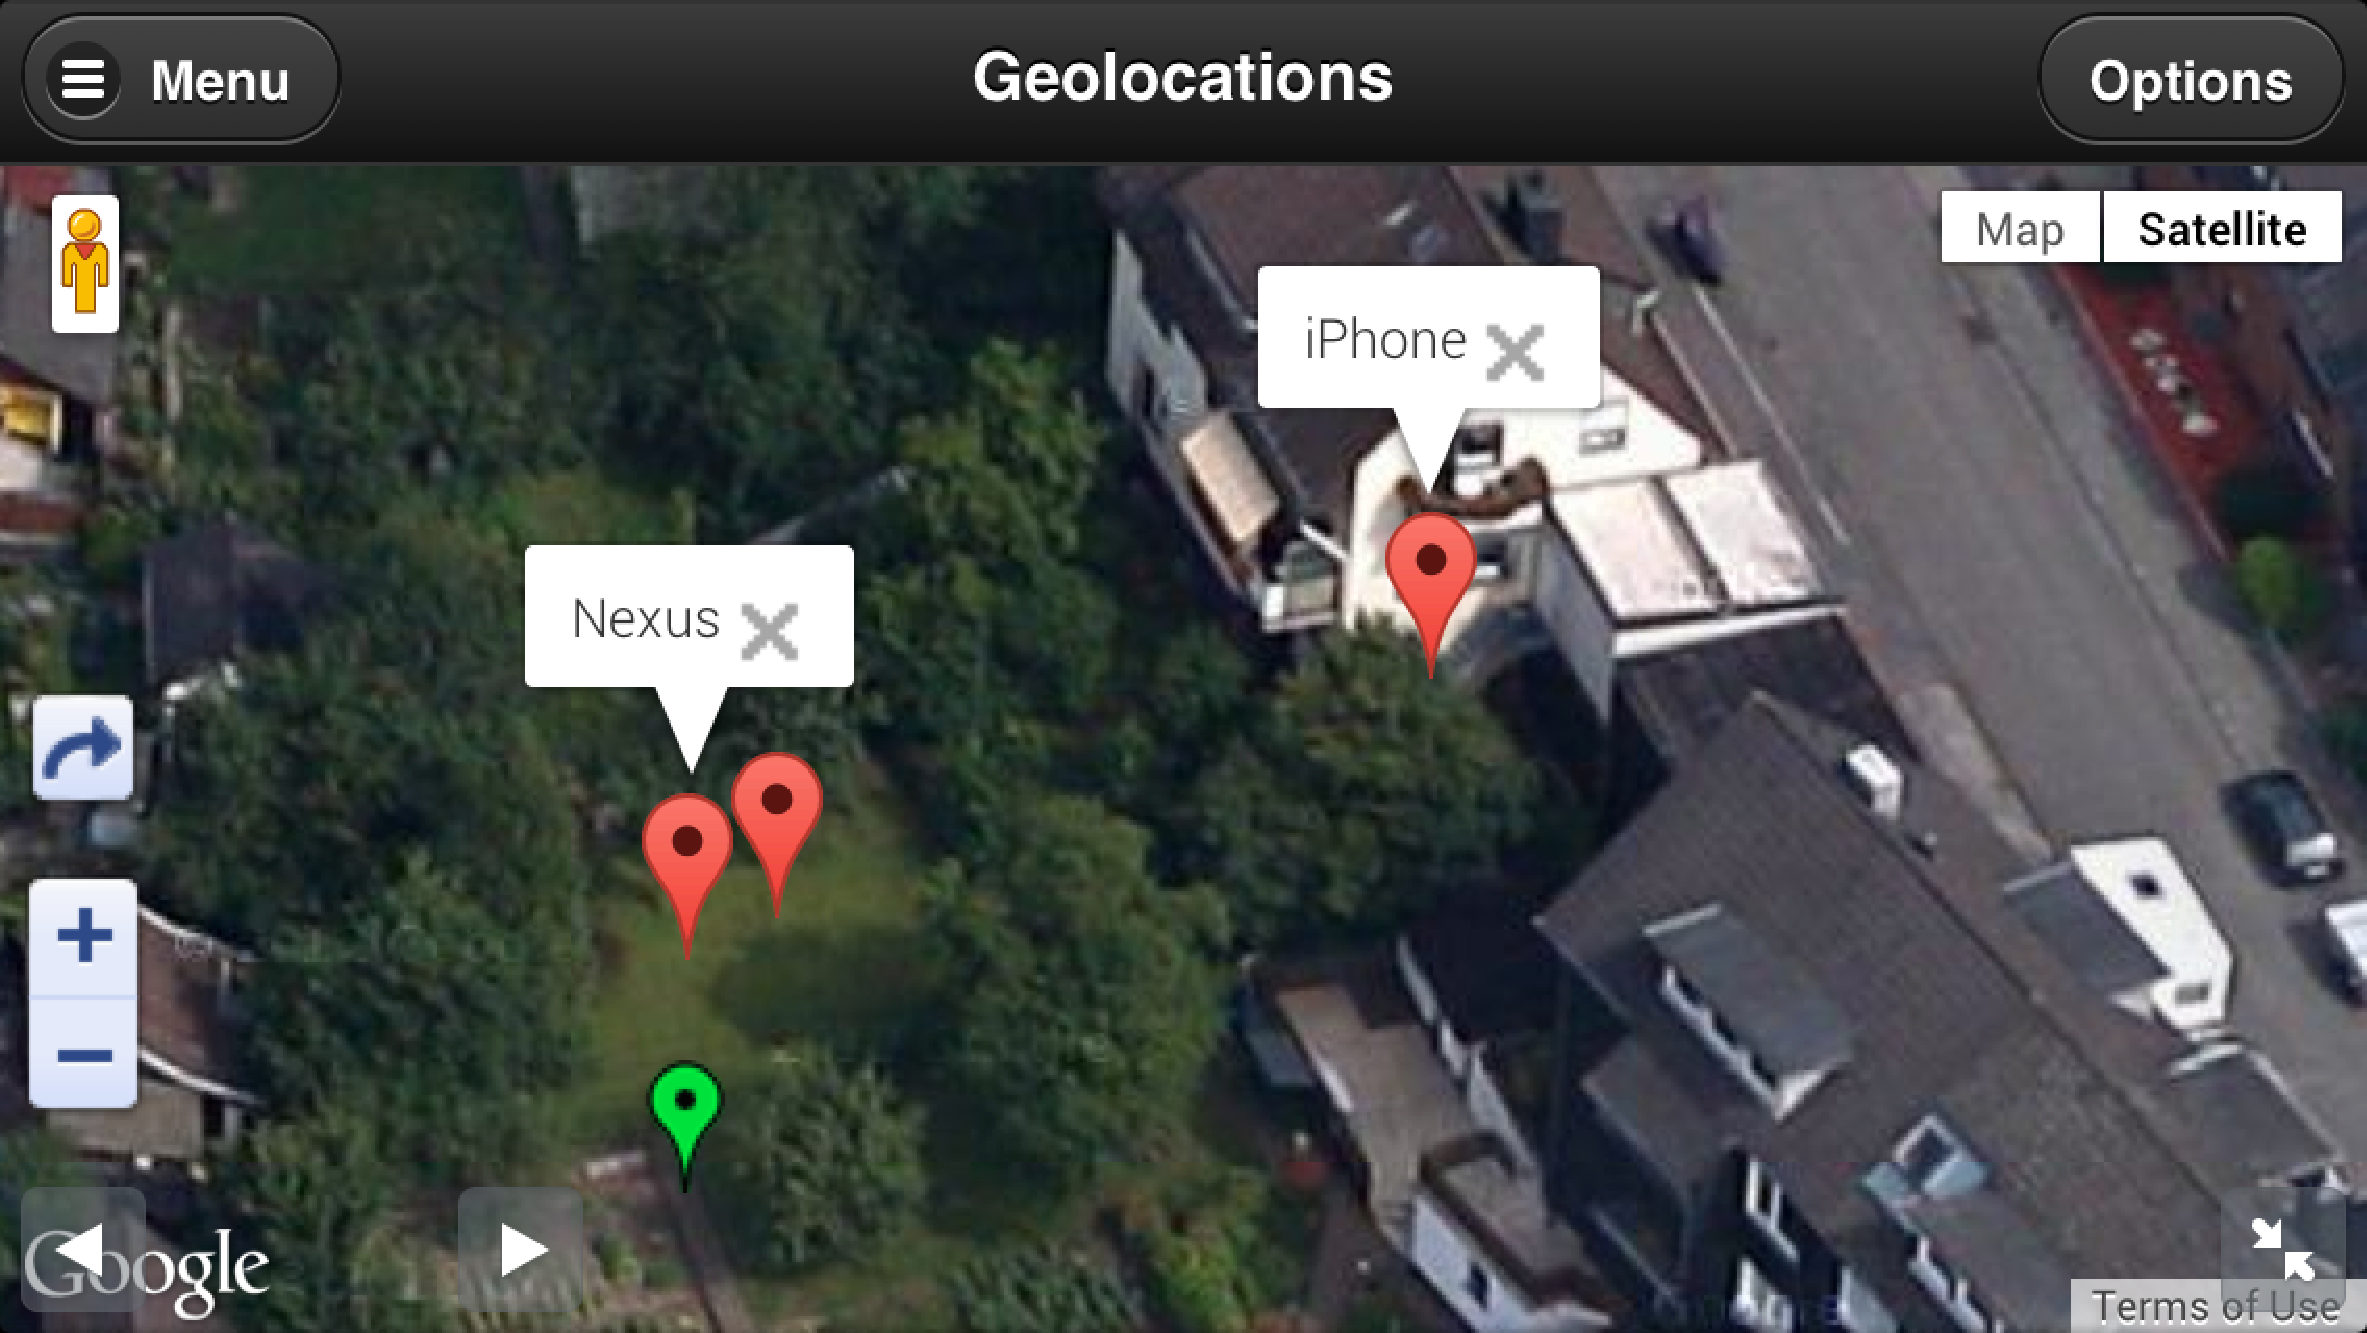
\includegraphics[width=15cm]{fig/screenshot_geolocations}
	\caption[Beispielansicht der Geolocations]{Getestet unter iOS 6.1.4, iPhone 5, Safari: Grün markiert eigene Position. Durch Tippen auf andere Marker erscheint der Name des Benutzers}
\end{figure}

Jeder Client kann auf diese Weise die Positionen der anderen Helfer sehen. Der Vorteil liegt klar auf der Hand: eine zentral eingerichtete Verwaltung kann mit einem Blick sehen, wer sich an welcher Stelle auf dem Gelände befindet. So können Wege optimiert und gezielt Aufgaben an sogenannte Springer verteilt werden, da ortsnahe Helfer die entsprechenden Aufgaben übernehmen können. Die kurzen Wege sorgen dann dafür, dass eine höhere Nutzung der Ressourcen (hier: die Helfer) möglich ist.\par

\paragraph{Anforderungen}
Eine wichtige Anforderung an diese Funktion ist, dass die Daten schnell ausgetauscht werden. Wenn zwischen den Updates der Geolocations zu viel Zeit vergeht, ist die Position nicht mehr aktuell und damit nicht mehr relevant. Deswegen findet der Austausch von Longitude und Latitude auch über WebSockets statt.

\paragraph{Kein Speichern der Positionsdaten}
Beendet ein Client die Verbindung oder erhält der Server keine Aktualisierungen mehr, so wird sein letzter Standort noch 15 Minuten gespeichert und dann auf allen Endgeräten gelöscht. Zu keiner Zeit werden Daten protokolliert oder länger als nötig aufbewahrt.

\subsection{Umgebungsbedingte Einschränkungen}
Bei diesem Projekt handelt es sich um eine Webanwendung, die aufgrund von Sicherheitsvorkehrungen einigen Einschränkungen unterliegt. So erlauben die mobilen Betriebssysteme keine Geopositionierung durch den Browser, wenn dieser minimiert ist oder das Smartphone / Tablet nicht aktiv genutzt wird. Das bedeutet, dass die Meißner App geöffnet sein muss, damit alle Funktionen genutzt und aktualisiert werden können.\par

Das ist für die Lokalisierung problematisch, da so die Position des Clients nicht aktuell bleibt. Diese Sicherheitsmaßnahmen sind jedoch sehr sinnvoll, denn es wäre sehr bedenklich könnte eine Homepage im Hintergrund stetig die Position des Besuchers überwachen. Allerdings genügt es, wenn die Webanwendung in einem Tab geöffnet ist, welcher nicht aktiv sein muss, um die Position des Endgeräts zu erfahren.

%%%%%%%%%%%%%%%%%%%%%%%%%%%%%%%%%%%%%%%%%%%%%%%%%%

\section{Offline-Funktionalität}
Mit der HTML5-Spezifikation wurde die \emph{Application Cache API} eingeführt, welche es ermöglicht, bestimmte Dateien einer Webanwendung in einen lokalen Cache zu speichern \cite[S. 189f]{friberg2013web}. Dafür ist eine \emph{Manifest}-Datei notwendig, die eine Liste mit den zu cachenden Dateien erstellt. Findet ein Browser ein Manifest, so lädt er initial die Webseite und speichert dabei alle Dateien in seinem Cache. Dieser ist bei normalen Anwendungen auf 5 MB beschränkt. Das reicht aber in der Regel vollkommen aus.\par

Die Meißner App generiert dynamisch mit jedem Aufruf der Anwendung ein Manifest, in der alle relevanten JavaScript Files, Bilder oder PHP-Seiten aufgeführt sind \cite{dynamic:manifest}. Dadurch kann die App erweitert werden, ohne die Offlinefunktion überarbeiten zu müssen.

\paragraph{Update des Caches}
Wurde die Anwendung einmal geladen und gecacht, so zeigt sie immer diesen Stand der Seite an. Damit der Browser aber angeregt wird die Seite neu zu cachen, muss eine Änderung am Manifest vorliegen. Das geschieht über eine Versionsnummer innerhalb dieser Datei: werden Änderungen an der Datenbank vorgenommen, dann inkrementiert die Webanwendung diese Nummer. Erreicht sie die Zahl 1000, so beginnt die Versionsnummer wieder bei 0.\par

Dadurch ist die Anwendung nun großteils offline verfügbar. Funktionen, wie die Geolocations oder der Chat, können allerdings nicht einwandfrei genutzt werden ohne Internetanbindung. Das liegt zum einen daran, dass Google das Cachen von Google Maps im Allgemeinen für Webanwendungen verbietet \cite{google:mapsforbidden} und daher die Offlineverwendung der Karte nicht möglich ist. Zum anderen ist für den Chat eine WebSocket-Verbindung notwendig, da sonst keine Nachrichten ausgetauscht werden können.\\
Mit gewissen Einschränkungen kann die Meißner App auch dort verwendet werden, wo nur eine schlechte Verbindung zur Verfügung steht. In jedem Fall lädt die App aber nun schneller, da sie nicht mehr alle Daten vom Webserver beziehen muss.

%%%%%%%%%%%%%%%%%%%%%%%%%%%%%%%%%%%%%%%%%%%%%%%%%%

\section{Installation auf einem Debian-basiertem  System}
Um diese Webanwendung mit sämtlichen Funktionen benutzen zu können, wurde eine einfache Installationsdatei in Form eines Shell-Scripts entwickelt. Dieses Skript downloadet und installiert als Webserver Apache2, MySQL und PHP5, danach wird die aktuellste Version von node.js gedownloadet und compiliert. Zuletzt wird die Meißner App in das Verzeichnis \emph{/var/www/meissner} verschoben, damit Apache2 darauf zugreifen kann.\par

Diese Installation wurde für ein unverändertes Debian 7 entwickelt und alle Abhängigkeiten, die für die Installation eines Webservers und WebSocket Servers notwendig sind, werden beachtet. Unter anderen debianbasierten Distributionen, wie Linux Mint, Ubuntu, etc., wurde das Skript auch erfolgreich getestet. Notwendig ist lediglich eine funktionierende Internetverbindung, da das Betriebssystem gleichzeitig noch aktualisiert und die aktuellste Version von node.js gedownloadet wird.\par

Abschließend erfolgt die Einrichtung der MySQL Datenbank über das Webinterface und kann unter \emph{http://localhost/meissner/setup} erreicht werden. Die Zugangsdaten zur gewünschten Datenbank müssen dort eingegeben werden und daraus fertig die Anwendung eine Konfigurationsdatei an, die sämtliche Informationen zur Verbindung mit der Datenbank enthält.\par

Alle Änderungen an der \emph{apache2.conf} und \emph{php.ini} werden automatisch eingefügt, sollten sie nicht schon standardmäßig installiert sein. Dabei handelt es sich in erster Linie um das Modul \emph{rewrite}, welches in den genannten Dateien geladen werden muss. Dieses Modul ermöglicht die Verwendung von kurzen URIs, die in dieser Anwendung verwendet werden. Das heißt der Benutzer kann in der Adressleiste des Browsers Links eingeben wie \emph{http://localhost/meissner/events} und wird sofort in die richtige Sektion weitergeleitet. Kryptische URIs werden so verhindert.

\paragraph{ReadMe}
Eine Installationsanleitung liegt separat zu der Meißner App bei. Da während der Installation der notwendigen Pakete einige Benutzereingaben notwendig sind, werden diese in Form von Bildschirmfotos erklärt. So ist eine verständliche Einrichtung der Anwendung möglich.

%%%%%%%%%%%%%%%%%%%%%%%%%%%%%%%%%%%%%%%%%%%%%%%%%%

% \section{Analyse der Skalierbarkeit}
% An den Webserver auf Apache-Basis o.Ä. werden mit der Meißner-App keine hohen Anforderungen gestellt, da ressourcenschonend entwickelt wurde und nur wenige SQL-Querys nötig sind für die Anzeige der Views. Interessanter ist allerdings die Echtzeitaktualisierung, da diese mit steigender Anzahl von Endgeräten deutlich mehr Sockets verwalten und mit Updates beliefern muss.

% \subsection{Zeitliches vs. konditionelles Update}
% Die \emph{navigator.geolocation} Klasse bietet mehrere Möglichkeiten seine Position zu aktualisieren. Jede Option wurde in Erwägung gezogen, die Zugriffe gemessen und schließlich in einer Tabelle ausgewertet. Die Auswertung ist daher interessant, weil die Skalierbarkeit dieser App noch nicht betrachtet wurde.\par

% Mit einbauen: http://hacks.mozilla.org/2009/06/geolocation/\par

% Die Statistiken hier baue ich noch ein...

%%%%%%%%%%%%%%%%%%%%%%%%%%%%%%%%%%%%%%%%%%%%%%%%%%

\section{Paketierung für App-Stores}
Auch bei Web-Apps besteht die Möglichkeit diese in den gängigen App-Stores wie dem von Apple oder Googles Play Store anzubieten. Dafür gibt es einige Frameworks, welche die eigentliche Webanwendung in eine Browserumgebung verpacken und diese dann wie eine native App aussehen lassen.\par
Für diese Arbeit wurde bewusst nicht darauf eingegangen und auch keine Paketierung für die Stores eingeplant. Das gesamte Projekt soll sehr dynamisch sein und ohne Grenzen der Stores für alle Geräte zur freien Verfügung stehen. Und eine Webseite aufrufen ist da die einfachste Möglichkeit die Anwendung zu nutzen.

\paragraph{Vorteile}
So können Änderungen an der Meißner App vorgenommen werden ohne, dass man kompliziert über die Stores die App neu verteilen muss. Außerdem ist absolut keine Installation notwendig, da sie wie eine normale Homepage geladen wird. Der Benutzer ist zwar nicht zwangsläufig gewohnt Apps über einen anderen Weg als den bekannten Store zu beziehen, aber da die Web-App genau so einfach geöffnet wird wie der Aufruf einer Homepage, kann man davon absehen.

\subsection{Add to Homescreen}
Bei Geräten mit dem Betriebssystem iOS ist die Funktion \emph{Add to Homescreen} verfügbar, welche eine Verknüpfung zur Webanwendung auf dem Homescreen erstellt. So kann die Anwendung wie eine normale App gestartet werden.\\
Durch eine einfache Ergänzung im Header der mobilen HTML Seite wird so eine appähnliche Installation ermöglicht.
\newpage
\begin{lstlisting}[captionpos=b, caption=Ergänzung im Header der mobilen Seite]
  <meta name="apple-mobile-web-app-capable" content="yes">
  <meta name="apple-mobile-web-app-status-bar-style"
  	content="black">
  <link rel="apple-touch-icon" href="img/icon.png">
\end{lstlisting}
Mit diesen drei Zeilen wird zuerst die Option \emph{Add to Homescreen} erlaubt, dann die Statusleiste schwarz gefärbt und der Pfad zum Icon angegeben, welches dann auf dem Homescreen erscheinen soll.\par

Das stellt eine einfache Möglichkeit dar eine Web-App zu installieren, allerdings gibt es keine ähnliche Funktion unter anderen Betriebssystemen wie Android o.Ä..

%%%%%%%%%%%%%%%%%%%%%%%%%%%%%%%%%%%%%%%%%%%%%%%%%%

\section{PUSH-Benachrichtigungen}
Bei Webanwendungen gibt es noch weitere Einschränkungen. So konnte für diese Arbeit nicht auf die systemeigenen Benachrichtigungsmechanismen zurückgegriffen werden, wie man sie aus nativen Applikationen her kennt. In den aktuellen Versionen aller mobilen Betriebssystemen sind Bereiche für Benachrichtigungen aus den jeweiligen Anwendungen implementiert um dem Benutzer zu signalisieren, dass neue Nachrichten vorliegen. Allerdings darf eine Web-App darauf nicht zugreifen, daher wurden für diese Anwendung eigene Methoden auf Basis von \emph{noty} \cite{noty}, einem jQuery Plugin für Benachrichtigungen, implementiert. Mit dieser Bibliothek wurde eine Benachrichtigungsleiste entwickelt, die am unteren Bildschirmrand Informationen anzeigen kann, wie zum Beispiel die oben angesprochene publish-Benachrichtigung vom WebSocket Server.\par

Auf diese Weise können nun auf allen Plattformen, die JavaScript aktiviert haben, Push-Benachrichtigungen angezeigt werden, wenn relevante Informationen über die WebSockets an das Endgerät gelangen.

%%%%%%%%%%%%%%%%%%%%%%%%%%%%%%%%%%%%%%%%%%%%%%%%%%

\section{Statistiken}
Da eine Auswertung der eingegebenen Daten für Veranstaltungen unabdinglich ist, wurde ein weiterer Controller implementiert, welcher sämtliche speziellen Felder der Events aus der Datenbank abfragt und diesen dann die Werte der einzelnen Benutzer zuweist.\par

Im View wird dann eine grafische Auswertung gestartet, die mit Hilfe von \emph{Google Charts} \cite{google:charts} ansehnliche Graphen mit JavaScript generiert, wo es Sinn ergibt und vergleichbare Werte von den Benutzern hinterlegt wurden. Außerdem gibt es allgemeine Statistiken, die die Veranstaltungen untereinander vergleichen und man so einen schnellen Überblick über die angelegten Events erhält.

\section{Chatfunktion}
Zur Kommunikation der Clients untereinander wurde der Bereich \emph{Chats} hinzugefügt. Der Datenaustausch findet über WebSockets statt und es ist keine weitere Konfiguration notwendig. Es muss nur der entsprechende View geöffnet werden, die Webanwendung erfragt die Historie beim WS Server und zeigt sie an. Ein einfaches Eingabeformular ermöglicht dann die Kommunikation mit allen eingeloggten Benutzern.

\begin{figure}[!ht]
	\centering
	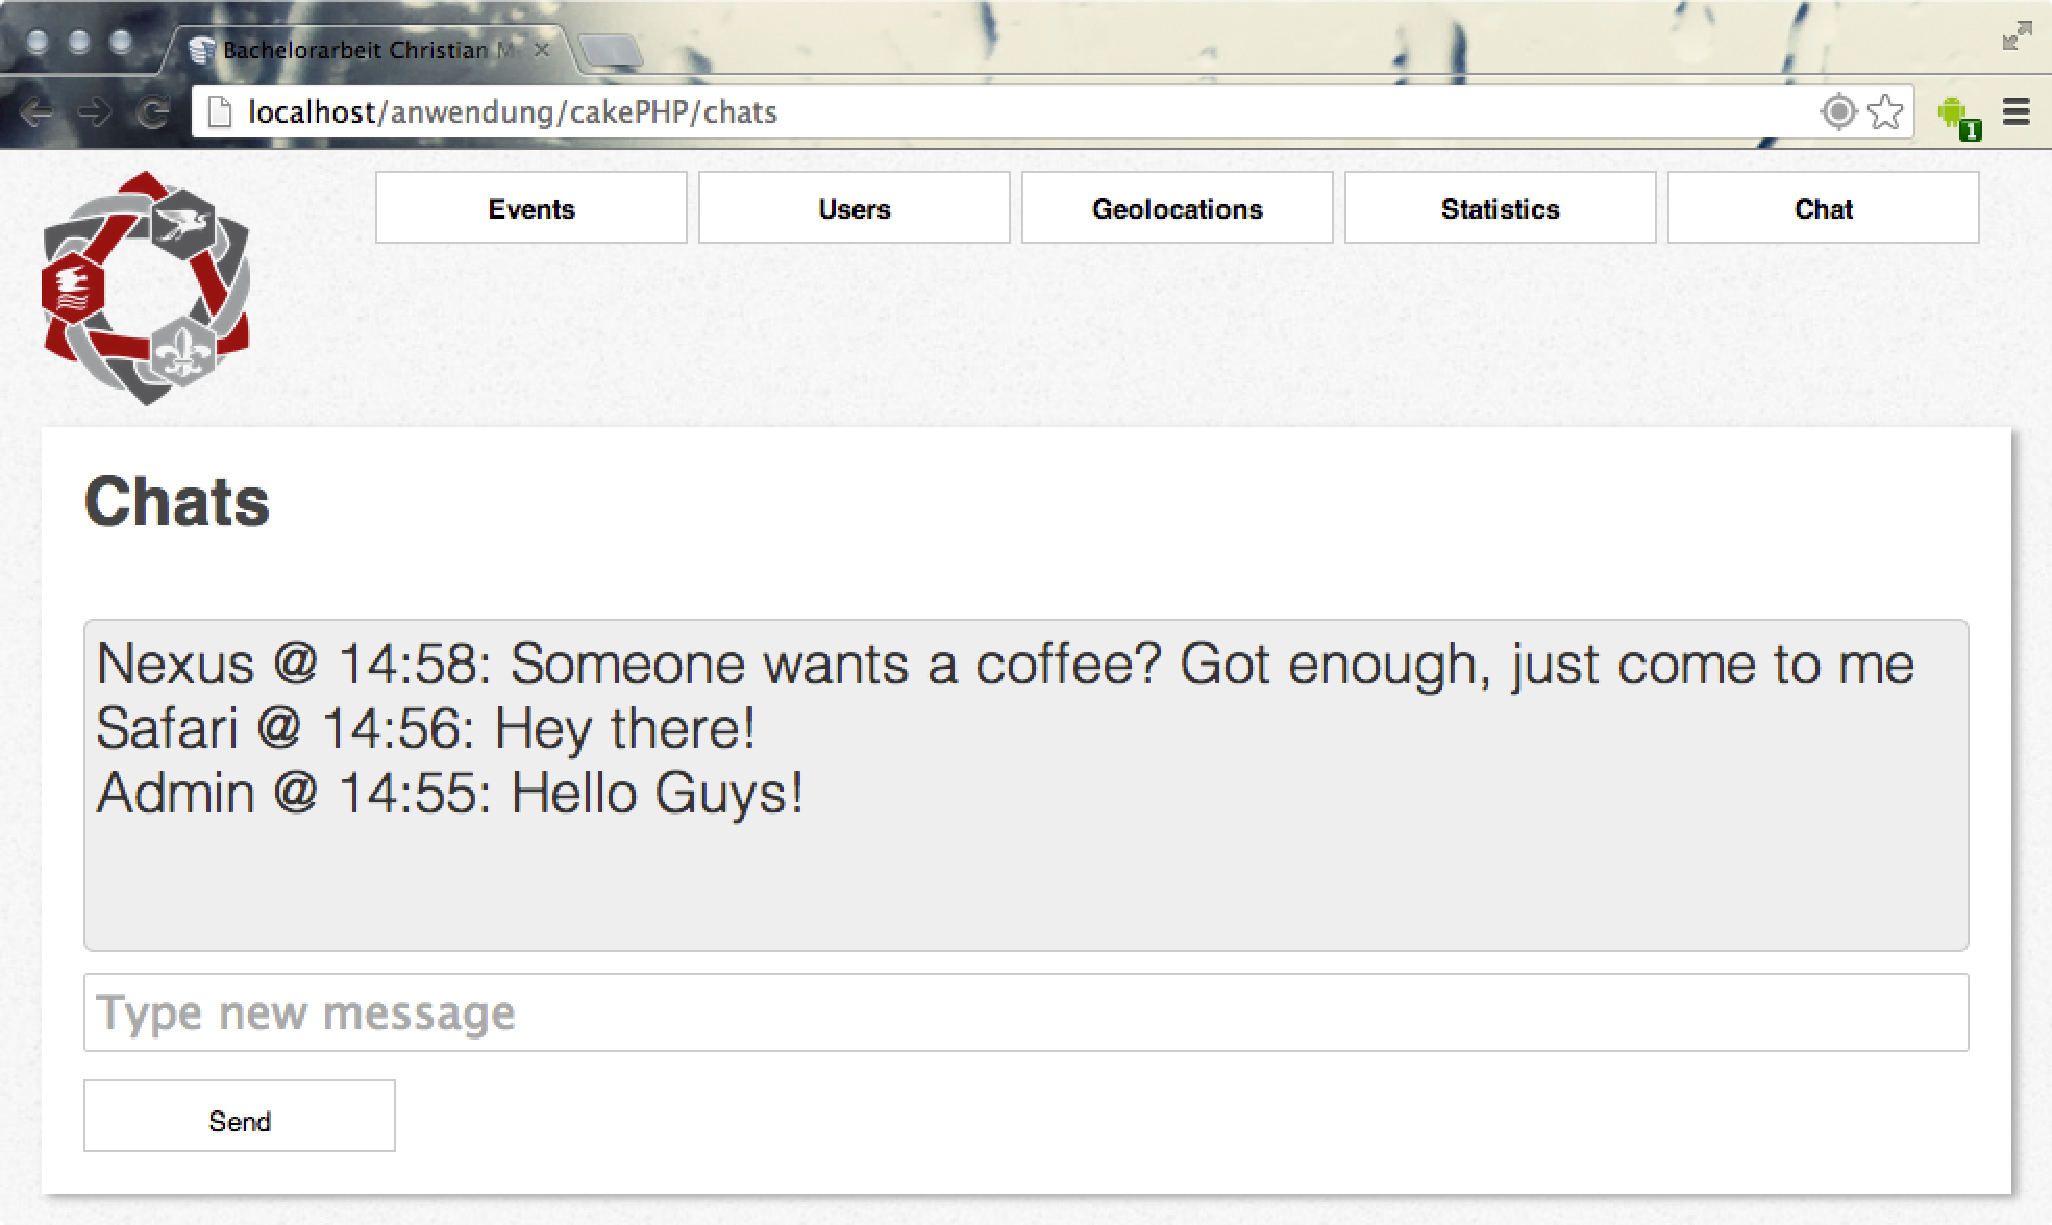
\includegraphics[width=15cm]{fig/screenshot_chat}
	\caption[Beispielansicht der Chats]{Getestet unter OS X 10.8.5., Chrome 29: Chatverlauf von drei verschiedenen Benutzern}
\end{figure}

Hierbei wird wieder Publish / Subscribe verwendet: Befindet sich ein Endgerät gerade im View des Chats, so abonniert die Webanwendung automatisch den Chat beim WebSocket Server und erhält dadurch alle eingehenden Nachrichten.

%%%%%%%%%%%%%%%%%%%%%%%%%%%%%%%%%%%%%%%%%%%%%%%%%%

%%%%%%%%%%%%%%%%%%%%%%%%%%%%%%%%%%%%%%%%%%%%%%
%%    End of the main document              %%
%%%%%%%%%%%%%%%%%%%%%%%%%%%%%%%%%%%%%%%%%%%%%%

\backmatter

\bibliographystyle{alphadin} %% german output

\bibliography{bachelor}

\printindex

\include{declaration}

\cleardoublepage

\chapter*{}
\thispagestyle{empty}

\begin{center}
  \vspace{-3cm}
  \fbox{\parbox[c][12cm][c]{12cm}{\centering Hier die H\"ulle\\[1cm]mit der CD/DVD einkleben}}
\end{center}

\vfill

\textbf{Diese CD enthält:}
\begin{itemize}
 \item eine \emph{pdf}-Version der vorliegenden Bachelorarbeit
 \item die \LaTeX- und Grafik-Quelldateien der vorliegenden Bachelorarbeit samt aller verwendeten Skripte
 \item die Quelldateien der im Rahmen der Bachelorarbeit erstellten Software \emph{Meißner App} unter \emph{anwendung/meissner}
 \item den zur Auswertung verwendeten Datensatz im Ordner \emph{anwendung/benchmark}
 \item die Websites der verwendeten Internetquellen im Ordner \emph{arbeit/Quellen}
\end{itemize}

\end{document}

